%==============================================================================%
\section{Antecedentes}

Marcano, Juan. $"$Implementaci�n de sistema de programaci�n de Trayectorias para el brazo manipulador MA2000". Universidad Central de Venezuela, 2013. Tutor: Prof. Alejandro Gonz�lez. Para establecer el control de posici�n del MA2000, se implement� un controlador de posici�n PID independiente para tres articulaciones utilizando el motor DSP de un dsPIC. Se desarroll� un software en el PC que se comunica con el microcontrolador y permite el ajuste din�mico del controlador PID y la visualizaci�n de la respuesta din�mica de cada articulaci�n as� como la programaci�n de trayectorias. Se ha recuperado el funcionamiento de la pinza neum�tica del equipo y se ha elaborado documentaci�n en l�nea del proyecto. \citep{juan1}

%==============================================================================%

Labrador, Alexis. "Dise�o de un equipo para el control y monitoreo de un motor asincr�nico usando una aplicaci�n m�vil". Universidad Central de Venezuela, 2018. Tutor: Prof. Servando �lvarez.El presente trabajo reporta el dise�o de un equipo para controlar el encendido y apagado, junto al monitoreo de tensi�n, corriente y tiempo de funcionamiento de un motor asincr�nico usando un ordenador de placa reducida y un dispositivo m�vil por medio de la red de comunicaci�n Internet de las cosas. Para lograrlo se selecciona el ordenador de placa reducida Raspberry Pi 3 modelo B, el sensor ACS712, m�dulos de rel�s para el accionamiento y componentes electr�nicos, se elige y se programa la plataforma de IoT, Ubidots for Education, para el monitoreo y control de forma remota, se selecciona la arquitectura de red en estrella, se eligen los tipos y modo de avisos que tendr� el sistema seg�n las que permite Ubidots for Education, para finalmente implementar dicho dise�o con el fin de validar el correcto funcionamiento.\citep{alexis1}

\section{Fundamentos sobre brazos manipuladores.}
\subsection{Brazo manipulador.}

Un brazo manipulador, o com�nmente llamado "brazo robot", es un sistema electr�nico programado para realizar acciones de control a una parte mec�nica. Estos existen de diversos tipos y morfolog�as y tienen m�ltiples aplicaciones industriales.\\
El t�rmino "brazo" se le atribuye por su similitud a la extremidad humana y a su funcionalidad. Contando en algunos casos con partes como "codo", "mu�eca", "hombro", "mano", entre otros. %Debido a que estos se dise�an para satisfacer una necesidad humana.
Existen de tipo: esf�rico, articulado, SCARA, cil�ndrico y cartesiano. Como se observa en la figura \ref{fig:tiporobot}.
\begin{figure}[H]
	\centering
	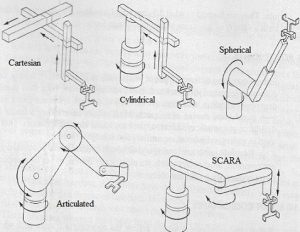
\includegraphics[scale=1]{img/tiporobot}
	\caption[Eckovation]{https://engineering.eckovation.com/pick-place-robotic-arm/}
	\label{fig:tiporobot}
\end{figure}


Entre algunos brazos manipuladores conocidos se tienen: PUMA 560, Stanford, Canadarm y Canadarm 2.

\subsection{Brazo pick and place.}

El t�rmino "pick and place" est� asociado a la utilidad del brazo rob�tico. Ya que posee un elemento final que permite sostener y soltar un elemento deseado. Seg�n la figura \ref{fig:tiporobot} cualquier tipo de brazo robot puede ser utilizado como pick and place, ya que no depende de sus grados de libertad ni de uniones, sino de poseer un elemento como una pinza o garra para cumplir una funci�n espec�fica.

Los siguientes brazos manipuladores a describir, se consideran del tipo "pick and place" debido a sus funciones.

\subsection{PUMA 560.}

\subsection{Stanford.}

\subsection{Canadarm y Canadarm 2.}

\subsection{Brazo manipulador MA2000.}

\section{Acceso remoto.}
\subsection{Acceso remoto por Bluetooth.}
\subsection{Acceso remoto por Wi-Fi.}
\subsection{Acceso remoto por RF.}
\subsection{LEGO MindStorm NXT.}
\subsection{Aplicaci�n de IoT.}
